\chapter{Iterazione 1}

\section{Introduzione}
Nella prima iterazione si è scelto di implementare i seguenti casi d'uso:

\begin{itemize}
    \item UC1: Gestione barche \textit{[Astratto]}
          \begin{itemize}
              \item UC1.1 Visualizzazione barche
              \item UC1.2 Inserimento barca
              \item UC1.3 Modifica barca
              \item UC1.4 Eliminazione barca
          \end{itemize}
    \item UC2: Gestione calendario uscite \textit{[Astratto]}
          \begin{itemize}
              \item UC2.1 Visualizzazione uscite
              \item UC2.2 Inserimento uscita
              \item UC2.3 Modifica uscita
              \item UC2.4 Eliminazione uscita
          \end{itemize}
    \item UC3: Registrazione utente
    \item UC4: Login utente
\end{itemize}
Dopo averli descritti in maniera testuale si è passati alla realizzazione del diagramma dei componenti e del deployment diagram.
Infine il codice è stato implementato sulla base di questi documenti.

\section{UC1: Gestione barche}

\emph{Breve descrizione}: il proprietario del diving center deve avere una visione generale e un controllo completo delle sue barche all'interno dell'applicazione.
Oltre alla visualizzazione, il proprietario deve poter modificare ed eliminare le imbarcazioni già presenti nel sistema e poter aggiungerne di nuove.
La gestione delle barche è quindi suddivisa in 4 casi d'uso concreti:

\begin{itemize}
    \item UC1.1 Visualizzazione barche
    \item UC1.2 Inserimento barca
    \item UC1.3 Modifica barca
    \item UC1.4 Eliminazione barca
\end{itemize}

\noindent \emph{Attori coinvolti}: Proprietario, Sistema.\medbreak
\noindent \emph{Trigger}: login del proprietario avvenuto con successo.\medbreak
\noindent \emph{Postcondizione}: il proprietario dopo il login, viene indirizzato alla home page e può scegliere se cliccare uno dei button: \textit{Visualizza barche} o \textit{Aggiungi barca}. Il primo per visualizzare
tutte le barche inserite, il secondo per aggiungerne una nuova.\medbreak
\noindent \emph{Procedimento}:

\begin{enumerate}
    \item Proprietario effettua il login.
    \item Sistema mostra la pagina iniziale che comprende un button \textit{Visualizza barche} e un button \textit{Aggiungi barca} con cui il proprietario può concretamente gestire le sue barche.
\end{enumerate}

\subsection{UC1.1 Visualizzazione barche}

\noindent \emph{Breve descrizione}: Il proprietario visualizza le barche inserite nel sistema e le relative caratteristiche.\medbreak
\noindent \emph{Attori coinvolti}: Proprietario, Sistema.\medbreak
\noindent \emph{Trigger}: Il proprietario clicca il button \textit{Visualizza barche}.\medbreak
\noindent \emph{Postcondizione}: Il sistema mostra una vista con l'elenco delle barche.\medbreak
\noindent \emph{Procedimento}:

\begin{enumerate}
    \item Proprietario effettua il login
    \item Proprietario clicca il button \textit{Visualizza barche} presente nella home page.
    \item Sistema mostra l'elenco delle barche presenti nel database con le seguenti informazioni:
          \begin{itemize}
              \item Nome della barca
              \item Modello della barca
              \item Numero posti disponibili sulla barca
              \item Altre caratteristiche TODO
          \end{itemize}
    \item Per ogni item dell'elenco il proprietario può cliccare su \textit{Modifica barca} o \textit{Elimina barca} per modificare o eliminare una barca.
\end{enumerate}

\subsection{UC1.2 Inserimento barca}

\noindent \emph{Breve descrizione}: Il proprietario aggiunge una barca nel sistema. Questo viene fatto principalmente nella fase iniziale in cui il proprietario deve inserire
tutte le sue barche all'interno dell'applicazione e poi in seguito all'acquisto di nuove barche.\medbreak
\noindent \emph{Attori coinvolti}: Proprietario, Sistema.\medbreak
\noindent \emph{Trigger}: Il proprietario clicca il button \textit{Inserisci barca}.\medbreak
\noindent \emph{Postcondizione}: Il sistema mostra la nuova barca all'interno della pagina di visualizzazione delle barche.\medbreak
\noindent \emph{Procedimento}:

\begin{enumerate}
    \item Il proprietario si trova sulla home page e clicca il button \textit{Inserisci barca}.
    \item Sistema mostra un form in cui è possibile inserire i dati relativi alla barca.
    \item Proprietario riempie il form.
    \item Proprietario clicca su \textit{Conferma} per inserire la barca nel sistema.
    \item Il sistema mostra la nuova barca all'interno della pagina di visualizzazione delle barche.
\end{enumerate}

\subsection{UC1.3 Modifica barca}

\noindent \emph{Breve descrizione}: Il proprietario si trova sulla pagina di visualizzazione delle barche e clicca su un button o un'icona di modifica di una delle barche.
Tale modifica può essere dovuta a cambiamenti strutturali della barca, per esempio la riduzione del numero di posti disponibili.
\medbreak
\noindent \emph{Attori coinvolti}: Proprietario, Sistema.\medbreak
\noindent \emph{Trigger}: Il proprietario clicca il button o l'icona \textit{Modifica barca}.\medbreak
\noindent \emph{Postcondizione}: Il sistema mostra la barca modificata all'interno della pagina di visualizzazione delle barche.\medbreak
\noindent \emph{Procedimento}:

\begin{enumerate}
    \item Il proprietario si trova sulla pagina di visualizzazione delle barche e clicca su un button o un'icona di modifica di una delle barche.
    \item Sistema mostra una vista in cui è possibile modificare i dati relativi alla barca.
    \item Proprietario modifica i dati.
    \item Proprietario clicca su \textit{Conferma} per modificare i dati della barca.
    \item Il sistema mostra la barca aggiornata all'interno della pagina di visualizzazione delle barche.
\end{enumerate}

\subsection{UC1.4 Eliminazione barca}

\noindent \emph{Breve descrizione}: Il proprietario si trova sulla pagina di visualizzazione delle barche e clicca su un button o un'icona di eliminazione di una delle barche.
L'eliminazione può essere definitiva o temporanea. L'eliminazione è definitiva se la barca non è più agibile o perché viene sostituita da un'altra;
è temporanea nel caso in cui sia necessaria attività di manutenzione.\medbreak
\noindent \emph{Attori coinvolti}: Proprietario, Sistema.\medbreak
\noindent \emph{Trigger}: Il proprietario clicca il button o l'icona \textit{Elimina barca}.\medbreak
\noindent \emph{Postcondizione}: Il sistema mostra la pagina di visualizzazione delle barche in cui non comparirà la barca eliminata.\medbreak
\noindent \emph{Procedimento}:

\begin{enumerate}
    \item Il proprietario si trova sulla pagina di visualizzazione delle barche e clicca su un button o un'icona di eliminazione di una delle barche. Il proprietario deve inoltre
          scegliere se l'eliminazione è temporanea o definitiva.
    \item Sistema mostra un alert che avvisa il proprietario che l'azione è irreversibile.
    \item Il proprietario può scegliere se confermare l'eliminazione cliccando su \textit{Conferma} o annullare l'azione cliccando su \textit{Annulla}.
    \item Il sistema mostra la pagina di visualizzazione delle barche in cui non comparirà la barca eliminata se il proprietario ha scelto di eliminarla in maniera non temporanea.
          Se invece, la barca è stata eliminata temporaneamente, essa sarà sempre visibile nella pagina di visualizzazione delle barche, ma segnalando al proprietario che il sistema organizzerà
          le uscite senza tenere conto di quella barca.
\end{enumerate}

\section{UC2: Gestione calendario uscite}
L'applicazione deve poter semplificare la gestione e l'organizzazione delle uscite al proprietario del diving center.
L'applicazione deve fungere da calendario, mettendo a disposizione le seguenti funzionalità:

\begin{itemize}
    \item UC2.1 Visualizzazione uscite
    \item UC2.2 Inserimento uscita
    \item UC2.3 Modifica uscita
    \item UC2.4 Eliminazione uscita
\end{itemize}

\subsection{UC2.1 Visualizzazione uscite}

\noindent \emph{Breve descrizione}: Il proprietario visualizza le date e i turni in cui gli utenti possono prenotarsi.\medbreak
\noindent \emph{Attori coinvolti}: Proprietario, Sistema.\medbreak
\noindent \emph{Trigger}: Il proprietario clicca il button \textit{Visualizza uscite}.\medbreak
\noindent \emph{Postcondizione}: Il sistema mostra una vista con l'elenco delle uscite.\medbreak
\noindent \emph{Procedimento}:

\begin{enumerate}
    \item Proprietario effettua il login.
    \item Proprietario clicca il button \textit{Visualizza uscite} presente nella home page.
    \item Sistema mostra l'elenco delle uscite rese disponibili con le seguenti informazioni:
          \begin{itemize}
              \item Data dell'uscita.
              \item Orario di inizio uscita.
              \item Orario di fine uscita.
              \item Altro TODO
          \end{itemize}
    \item Per ogni data presente nell'elenco il proprietario può cliccare su \textit{Modifica uscita} o \textit{Elimina uscita} per modificare o eliminare un'uscita.
\end{enumerate}

\subsection{UC2.2 Inserimento uscita}

\noindent \emph{Breve descrizione}: Il proprietario aggiunge un'uscita al calendario indicandone data e orari in cui verranno rese disponibili le prenotazioni.\medbreak
\noindent \emph{Attori coinvolti}: Proprietario, Sistema.\medbreak
\noindent \emph{Trigger}: Il proprietario clicca il button \textit{Inserisci uscita}.\medbreak
\noindent \emph{Postcondizione}: Il sistema mostra la nuova uscita all'interno della pagina di visualizzazione delle uscite.\medbreak
\noindent \emph{Procedimento}:

\begin{enumerate}
    \item Il proprietario si trova sulla home page e clicca il button \textit{Inserisci uscita}.
    \item Sistema mostra un form in cui è possibile inserire i dati relativi all'uscita.
    \item Proprietario riempie il form.
    \item Proprietario clicca su \textit{Conferma} per inserire l'uscita nel sistema.
    \item Il sistema mostra la nuova uscita all'interno della pagina di visualizzazione delle uscite.
\end{enumerate}

\subsection{UC2.3 Modifica uscita}

\noindent \emph{Breve descrizione}: Il proprietario si trova sulla pagina di visualizzazione delle uscite e clicca su un button o un'icona di modifica di una delle uscite.
Tale modifica può essere dovuta a cambiamenti climatici o ad altri imprevisti.\medbreak
\noindent \emph{Attori coinvolti}: Proprietario, Sistema.\medbreak
\noindent \emph{Trigger}: Il proprietario clicca il button o l'icona \textit{Modifica uscita}.\medbreak
\noindent \emph{Postcondizione}: Il sistema mostra l'uscita modificata all'interno della pagina di visualizzazione delle uscite.\medbreak
\noindent \emph{Procedimento}:

\begin{enumerate}
    \item Il proprietario si trova sulla pagina di visualizzazione delle uscite e clicca su un button o un'icona di modifica di una delle uscite.
    \item Sistema mostra una vista in cui è possibile modificare i dati relativi all'uscita.
    \item Proprietario modifica i dati.
    \item Proprietario clicca su \textit{Conferma} per modificare i dati dell'uscita.
    \item Il sistema mostra l'uscita aggiornata all'interno della pagina di visualizzazione delle uscite.
\end{enumerate}

\subsection{UC2.4 Eliminazione uscita}

\noindent \emph{Breve descrizione}: Il proprietario si trova sulla pagina di visualizzazione delle uscite e clicca su un button o un'icona di eliminazione di una delle uscite.\medbreak
\noindent \emph{Attori coinvolti}: Proprietario, Sistema.\medbreak
\noindent \emph{Trigger}: Il proprietario clicca il button o l'icona \textit{Elimina uscita}.\medbreak
\noindent \emph{Postcondizione}: Il sistema mostra la pagina di visualizzazione delle uscite in cui non comparirà l'uscita eliminata.\medbreak
\noindent \emph{Procedimento}:

\begin{enumerate}
    \item Il proprietario si trova sulla pagina di visualizzazione delle uscite e clicca su un button o un'icona di eliminazione di una delle uscite.
    \item Sistema mostra un alert che avvisa il proprietario che l'azione è irreversibile.
    \item Il proprietario può scegliere se confermare l'eliminazione cliccando su \textit{Conferma} o annullare l'azione cliccando su \textit{Annulla}.
    \item Il sistema mostra la pagina di visualizzazione delle uscite in cui non comparirà l'uscita eliminata.
\end{enumerate}

\section{UC3: Registrazione dell'utente}
\noindent \emph{Breve descrizione}: L'utente compila il form per la registrazione all'app e, se non si è già registrato, viene aggiunto al database.\medbreak
\noindent \emph{Attori coinvolti}: Utente, Sistema?\medbreak
\noindent \emph{Trigger}: L'utente preme su "Registrazione".\medbreak
\noindent \emph{Postcondizione}: L'utente è stato inserito nel database e ha ricevuto la conferma dell'operazione.\medbreak
\noindent \emph{Procedimento}:
\begin{enumerate}
    \item Utente preme su "Registrazione" nella pagina iniziale dell'app
    \item Utente fornisce Nome, username, indirizzo email e password nel form di registrazione
    \item Il sistema verifica se esiste già un utente con quella mail:
          \begin{enumerate}
              \item se esiste già, il sistema lo comunica all'utente
              \item se non esiste allora il sistema aggiunge l'utente nel database
          \end{enumerate}
\end{enumerate}

\section{UC4: Login dell'utente}
\noindent \emph{Breve descrizione}: L'utente (utente normale o il proprietario) compila il form per il login e se le credenziali sono giuste il sistema gli consente l'accesso.\medbreak
\noindent \emph{Attori coinvolti}: Utente/Proprietario, Sistema?\medbreak
\noindent \emph{Trigger}: L'utente preme su "Login"\medbreak
\noindent \emph{Postcondizione}: L'utente ha accesso alla vista del suo profilo.\medbreak
\noindent \emph{Procedimento}:
\begin{enumerate}
    \item Utente preme su "Login" nella pagina iniziale dell'app
    \item Utente fornisce username e password nel form di registrazione
    \item Il sistema controlla le credenziali inserite:
          \begin{enumerate}
              \item se sono corrette, il sistema invia una conferma di accesso all'utente
              \item se sono errate, il sistema lo comunica all'utente
          \end{enumerate}
\end{enumerate}

\section{UML Component diagram}
I casi d'uso scelti in questa prima iterazione vengono rappresentati sottoforma di componenti nel diagramma in Figura~\ref{fig:componentDiagram}.
Si è scelto di suddividire i caso d'uso in componenti:

\begin{itemize}
    \item <<boundary>> rappresentati dai componenti lato front-end con cui gli attori si interfacciano direttamente. Tali componenti richiedono delle interfacce al back-end.
    \item <<control>> rappresentati dai componenti lato back-end che forniscono delle API al front-end, richiedonone a loro volta al database.
    \item <<data>> rappresentato dal database in cui verranno memorizzati i dati delle barche, il calendario delle uscite e i dati dell'utente in occasione della registrazione.
\end{itemize}

\begin{figure}
    \centering
    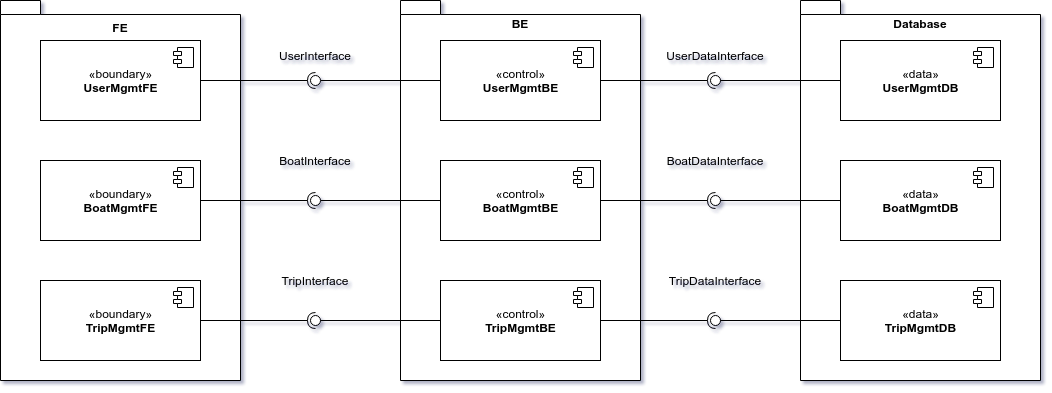
\includegraphics[width=\textwidth]{ComponentDiagram_v3.png}
    \caption{Diagramma dei componenti UML.}\label{fig:componentDiagram}
\end{figure}

\newpage

\section{UML Class diagram per Interfacce}
Il diagramma in Figura ~\ref{fig:ClassDiagramInterfaces} serve a rappresentare le interfacce del sistema e le loro interazioni.
\begin{figure}[hb]
    \centering
    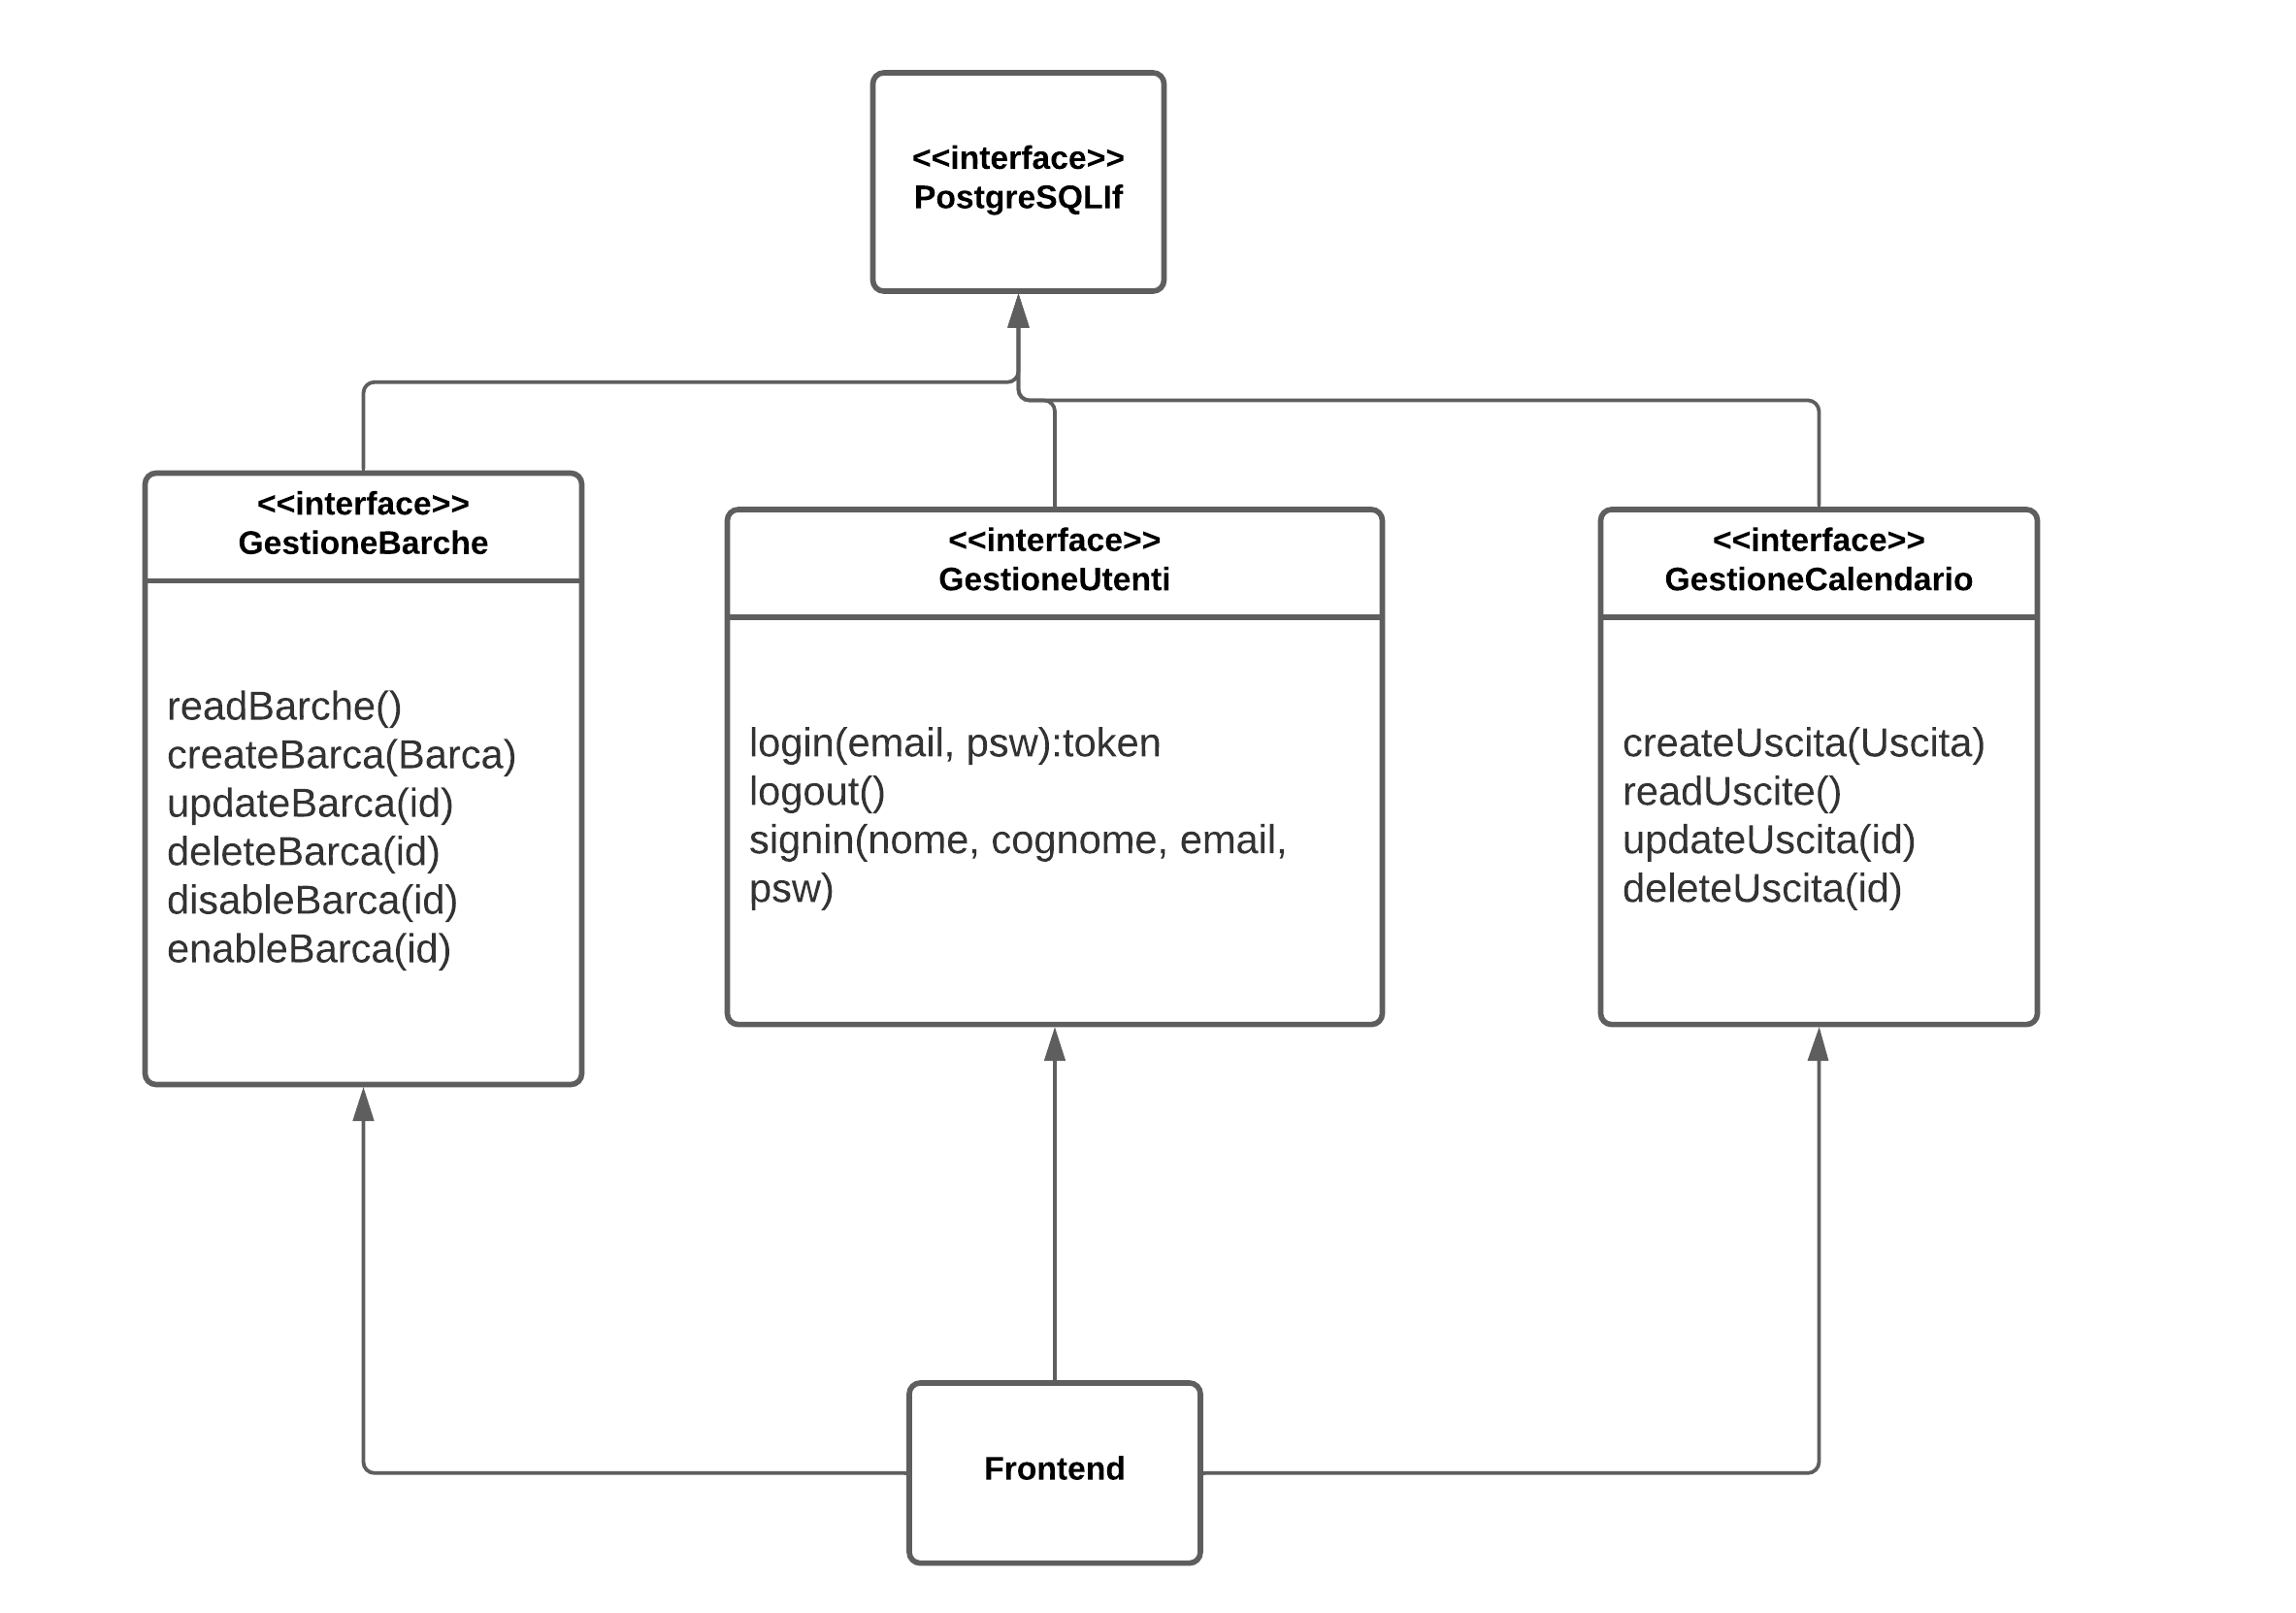
\includegraphics[width=\textwidth]{ClassDiagramInterfaces_v2.png}
    \caption{Diagramma dei componenti UML.}\label{fig:ClassDiagramInterfaces}
\end{figure}

\newpage

\section{UML Class diagram per tipi di dato}
Il seguente diagramma serve ad esplicitare tipi di dato particolari e i loro legami.
\begin{figure}[h]
    \centering
    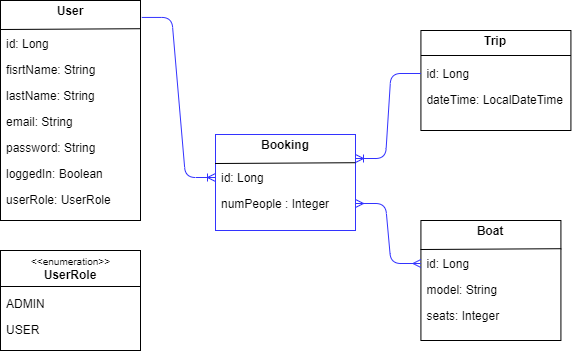
\includegraphics[width=\textwidth]{ClassDiagramTypes_v1.png}
    \caption{Diagramma dei componenti UML.}\label{fig:ClassDiagramTypes}
\end{figure}

\section{UML Deployment diagram}
I componenti descritti precedentemente vengono istanziati nel Deployment diagram. In Figura~\ref{fig:DeploymentDiagram} vengono mostrati i componenti contenuti nei seguenti nodi:

\begin{itemize}
    \item Cellulare proprietario è il nodo su cui l'admin del sistema potrà gestire le barche e il calendario delle uscite.
    \item Cellulare utente è il nodo su cui una persona potrà registrarsi alla piattaforma.
    \item Web server fornisce le API richieste dall'applicativo lato front-end.
    \item Database funge da storage dei dati.
\end{itemize}

\begin{figure}
    \centering
    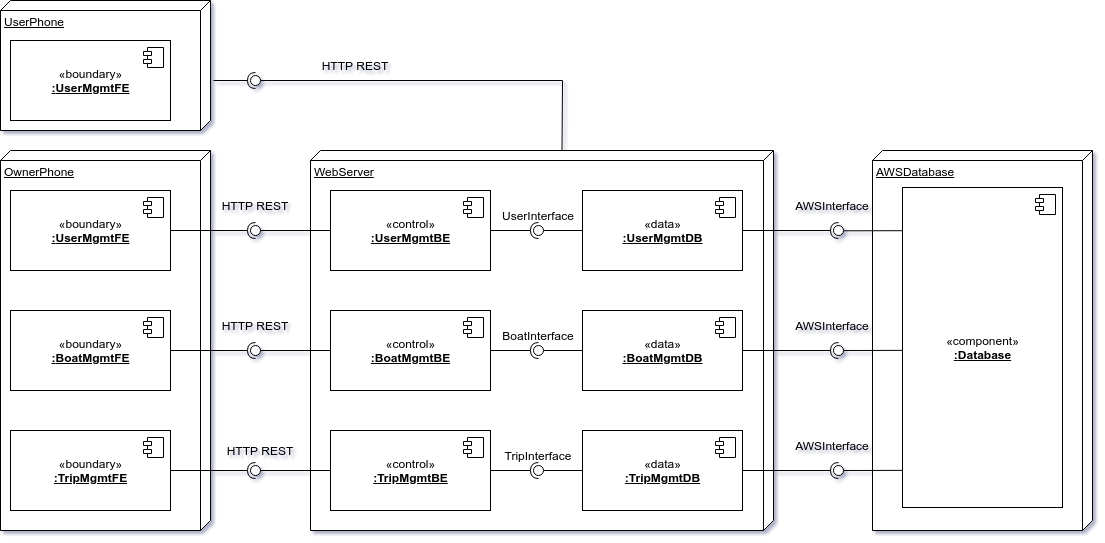
\includegraphics[width=\textwidth]{DeploymentDiagram_v5.png}
    \caption{Deployment diagram UML.}\label{fig:DeploymentDiagram}
\end{figure}